\documentclass[twoside]{article}

\usepackage[math]{kurier}
\usepackage[sc]{mathpazo} 
\usepackage{subcaption}
\usepackage{graphicx}
\usepackage[utf8]{inputenc}
\usepackage[T1]{fontenc}
\usepackage[export]{adjustbox}
\usepackage{color}
\usepackage{amsmath}

\renewcommand{\sfdefault}{kurier}


\usepackage{graphics}
\setlength{\oddsidemargin}{0.25 in}
\setlength{\evensidemargin}{-0.25 in}
\setlength{\topmargin}{-0.6 in}
\setlength{\textwidth}{6.5 in}
\setlength{\textheight}{8.5 in}
\setlength{\headsep}{0.75 in}
\setlength{\parindent}{0 in}
\setlength{\parskip}{0.1 in}


\newcounter{lecnum}
\renewcommand{\thepage}{\thelecnum-\arabic{page}}
\renewcommand{\thesection}{\thelecnum.\arabic{section}}
\renewcommand{\theequation}{\thelecnum.\arabic{equation}}
\renewcommand{\thefigure}{\thelecnum.\arabic{figure}}
\renewcommand{\thetable}{\thelecnum.\arabic{table}}


\newcommand{\lecture}[4]{
   \pagestyle{myheadings}
   \thispagestyle{plain}
   \newpage
   \setcounter{lecnum}{#1}
   \setcounter{page}{1}
   \noindent
   \begin{center}
   \framebox{
      \vbox{\vspace{2mm}
    \hbox to 6.28in { {\bf \sffamily AA 274: Principles of Robotic Autonomy
                        \hfill Winter 2018} }
       \vspace{4mm}
       \hbox to 6.28in { {\sffamily{\Large \hfill Lecture #1: #2  \hfill}} }
       \vspace{2mm}
       \hbox to 6.28in { {\it \hfill Scribes: #4} }
      \vspace{2mm}}
   }
   \end{center}
   \markboth{Lecture #1: #2}{Lecture #1: #2}

   \vspace*{4mm}
}



%%%%%%%%%%%%%%%%%%%%%%%%%%
%document
\begin{document}

\lecture{11}{Localization part 2 - Parametric and Non-Parametric Filters}{}{Steve Burke, Claire Huang, Emma Morgan, Eley Ng, Stephanie Schneider, Gareth Weiss}

\section{Introduction}
Successful robot navigation incorporates four fundamental building blocks:
\begin{itemize}
    \item Perception: extract data from sensors
    \item Localization: build a map and determine position within the environment
    \item Cognition: decide how to move towards end goal
    \item Motion control: actuate motors to move along chosen path
\end{itemize}

Lecture 11 completes the description of localization strategies. In Lecture 10, Bayes' Filter Algorithm was described in its general, incalculable form. Here, we introduce some tractable solutions used for real-world localization.

These solutions can be grouped into two methods: parametric and non-parametric. The parametric class of filters forces a predefined structure onto the problem. Non-parametric filters, on the other hand, make no assumption about structure, and therefore must introduce approximations to make the algorithm computationally feasible.
    
\section{Parametric Filters}\label{sec:parametric}

\subsection{Gaussian Distribution}\label{sec:gaussian}
In a Gaussian belief state, the belief is represented as a mutlivariate normal distribution, given by Equation \ref{eq:gaussdist}
\begin{equation}\label{eq:gaussdist}
    p(x) = det(2\pi\Sigma)^{-1/2}exp\Big{(}-\frac{1}{2}(x-\mu)^T\Sigma^{-1}(x-\mu)\Big{)} \rightarrow \mathcal{N}(\mu, \Sigma)
\end{equation}
The Gaussian distribution has a parametric density, meaning it is parameterized entirely by $\mu$ and $\Sigma$. Gausian distributions are also unimodal and symmetric about the mean. In the univariate case, the mean and variance are both scalar quantities; in the multidimensional generalization, the mean ($\mu$) is a vector of means, and the covariance ($\Sigma$) is a matrix. The covariance matrix tells us about the uncertainty of each random variable along every dimension. A multivariance Gaussian distribution can be visualized as a contour plot (as in Figure \ref{fig:NDgauss}), where density is constant along a given contour.

\begin{figure}[h]
    \begin{subfigure}{0.5\textwidth}
        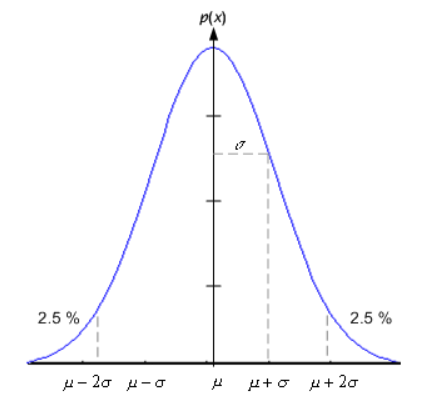
\includegraphics[width=0.9\linewidth, height=5cm]{scribe_1Dgauss} 
        \caption{Univariate Gaussian}
        \label{fig:1Dgauss}
    \end{subfigure}
    \begin{subfigure}{0.5\textwidth}
        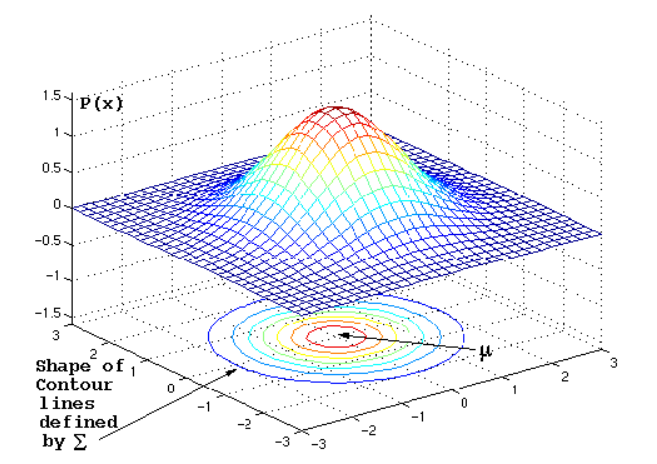
\includegraphics[width=0.9\linewidth, height=5cm]{scribe_nDgauss}
        \caption{Multivariate Gaussian}
        \label{fig:NDgauss}
    \end{subfigure}
\end{figure}
% ========== both images taken from here ==========
% https://www.byclb.com/TR/Tutorials/neural_networks/ch4_1.htm

Non-symmetric variance (e.g. a distribution with elliptical contours) can be explained by considering the example of a car. A self-driving car, which moves primarily in the forward/backward direction, will have more positional uncertainty in the longitudinal direction than laterally.

\subsubsection{Gaussian Properties}\label{sec:gaussProperties}
\begin{itemize}
    \item A linear transformation of a Gaussian random variable is a Gaussian random variable (see [\ref{bib:lecnotes}] for derivation)\\
    % ========== This was taking up a lot of space ================
    % \begin{tabular}{l c}
    %    Define a Gaussian RV: & $X \sim \mathcal{N}(\mu, \Sigma)$ \\
    %    Define linear transformation Y: & $Y = AX + b$ \\
    %     
    %\end{tabular}\\ \\
    %With any constant matrix A. Expected value is a linear operator, so if $Ex[X] = %\mu$, and $Ex[b] = b$ (b is a constant), then
    %$$Ex[Y] = A\mu + b$$
    %We know from Lecture 8 that the variance of a sum is equal to the sum of variances, %and that the variance of a constant is zero. So,
    %$$Var(AX) = E[(A(X-\mu))^2]$$
    %$$ = E[(A(X-\mu))(A(X-\mu))^T]$$
    %$$ = E[A(X-\mu)(X-\mu)^TA^T$$
    %$$ = AE[(X-\mu)(X-\mu)^T]A^T$$
    %$$ = AVar(X)A^T$$
    %
    %
    %Therefore,
    \begin{equation}
         Y = AX + b \sim \mathcal{N}\big{(}A\mu+b,  A\Sigma A^T\big{)}
    \end{equation}
    
    \item The sum of two independent Gaussian random variables is Gaussian
    \begin{equation}
        X_1 + X_2 \sim \mathcal{N}(\mu_1 + \mu_2, \Sigma_1 + \Sigma_1)
    \end{equation}
    
    \item The product of two independent Gaussian pdfs is Gaussian
    \begin{equation}
        X_1X_2 \sim \mathcal{N}\Big{(}\Sigma_2(\Sigma_1+\Sigma_2)^{-1}\mu_1 + \Sigma_1(\Sigma_1+\Sigma_2)^{-1}\mu_2,\ \Sigma_1(\Sigma_1+\Sigma_2)^{-1}\Sigma_2 \Big{)}
    \end{equation}
    
\end{itemize}

\subsection{Kalman Filters}
\subsubsection{Assumptions}
\begin{enumerate}
    \item Linear Dynamics
    $$ x_t = A_t x_{t-1} + B_t u_t + \epsilon_t$$
    where process noise is Gaussian ($\epsilon_t \sim \mathcal{N}(0, R_t)$).
    Considering $x_{t-1}$ and $u_t$ as givens (i.e. constants),  the state transition probability ($p(x_t | u_t, x_{t-1})$) is a linear transformation of only the Gaussian noise. Therefore, the posterior is also Gaussian, with mean = $A_t x_{t-1} + B_t u_t$, and variance equal to variance of process noise = $R_t$.
    
    \item Linear Measurement Model
    $$z_t = C_t x_t + \delta_t$$
    where process noise is Gaussian ($\delta_t \sim \mathcal{N}(0, Q_t)$).
    The posterior $p(z_t | x_t)$ in this case is also a linear transformation of the Gaussian process noise, with mean = $C_t x_t$, and variance = $Q_t$.
    
    \item Initial Belief is Gaussian
    $$ bel(x_0) = det(2\pi\Sigma_0)^{-\frac{1}{2}}exp\Big{(}-\frac{1}{2}(x_0 - \mu_0)^T\Sigma_0^{-1}(x_0 - \mu_0)\Big{)}$$
    
\end{enumerate}
By enforcing these three assumptions, and using the properties in Section \ref{sec:gaussProperties}, we can ensure that the posterior belief $bel(x_t)$ will always be Gaussian as well. We often use Gaussian assumptions even if they are invalid, in order to parameterize the problem and make it computationally feasible. This forces a unimodal belief, but is often a good approximation even for non-Gaussian data.

\subsubsection{Algorithm}
The Kalman filter algorithm follows the Bayes filter structure while dramatically simplifying computation by using Gaussians. It consists of two steps: prediction and correction. At some time $t$, we know the previous belief, defined by the two parameters $\mu_{t-1}$ and $\Sigma_{t-1}$,  the current control action $u_t$, and the measurement $z_t$. We want to update our belief and determine the current state $\mu_t$ and $\Sigma_t$. In the prediction step, we update our prediction of belief at time $t$ using a linear dynamics model. 
\begin{equation}
    \overline{\mu}_t = A_t \mu_{t-1} + B_t u_t
\end{equation}
\begin{equation}
    \overline{\Sigma}_t = A_t \Sigma_{t-1} A_t^T + R_t
\end{equation}

Once we have the predicted belief, we incorporate our current measurement to refine our belief in the correction step. We define an additional Kalman gain $K_t$ that weights our trust in the dynamic model versus trust in the measurement.
\begin{equation}
    K_t = \overline{\Sigma}_t C_t^T (C_t \overline{\Sigma}_t C_t^T + Q_t)^{-1}
\end{equation}
By this definition, $K_t$ grows inversely with our measurement uncertainty (the terms in the denominator) -- greater uncertainty means a smaller $K_t$. We then use the gain to calculate our final belief parameters:
\begin{equation}
    \mu_t = \overline{\mu}_t + K_t(z_t - C_t \overline{\mu}_t)
\end{equation}
\begin{equation}
    \Sigma_t = (I - K_t C_t) \overline{\Sigma_t}
\end{equation}

\subsection{Extended Kalman Filter}

\subsubsection{Linearity Assumption}
The most important property of the linearity assumption is that the linear transformation of a Gaussian random variable results in another Gaussian RV. The standard Kalman Filter algorithm relies on a linear transformation to propagate the state model forward, but unfortunately, this assumption of linear dynamics is severely restrictive for robotics applications.

\subsubsection{EKF Set-up}
The goal of the Extended KF is to relax the linearity assumptions, therefore making it more useful for robotics applications.  For the EKF, the dynamics and measurement models are given by:
\begin{equation}
    x_t = g(u_t,x_{t-1}) + {\epsilon}_t
\end{equation}
\begin{equation}
    z_t = h(x_t) + {\delta}_t
\end{equation}
The key idea is to use these equations to focus on efficiently computing a Gaussian approximation of the dynamics model, rather than finding an exact posterior. We do this by linearly approximating g and h around the most likely state. By using Jacobians ($G_t$ and $H_t$), we can take advantage of the non-linear generalizations of both the dynamics and the measurement models. This results in the following equations:
$$ p(x_t|u_t,x_{t-1}) =$$
\begin{equation}
    \det(2{\pi}R_t)^{-1/2}\exp((-1/2)[x_t - g(u_t,{\mu}_{t-1}) - G_t(x_t - {\mu}_{t-1})]^{T}R_t^{-1}[x_t - g(u_t,{\mu}_{t-1}) - G_t(x_{t-1} - {\mu}_{t-1})])
\end{equation}
\begin{equation}
    p(z_t|x_t) = \det(2{\pi}Q_t)^{-1}\exp((-1/2)[z_t - h(\overline{\mu}_t) - H_t(x_t - \overline{\mu}_t)]Q_t^{-1}[z_t - h(\overline{\mu}_t) - H_t(x_t - \overline{\mu}_t)])
\end{equation}
\subsubsection{Algorithm}
The main difference between the Kalman Filter and EKF is that the EKF uses non-linear generalizations, while the regular Kalman Filter models the dynamics using linear predictions. Mathematically, the EKF uses Jacobians instead of linear system matrices. Both algorithms follow the same high-level derivation, and both use the Bayesian structure of having a prediction step followed by a correction step.

The inputs for the EKF are:
\begin{itemize}
    \item ${\mu}_{t-1}$: expected value of the state at time $t-1$
    \item ${\Sigma}_{t-1}$: variance of the estimate at $t-1$
    \item $z_t$: measurement taken at time $t$
\end{itemize}

The EKF outputs a Gaussian approximation for the posterior belief, parameterized by ${\mu}_t$ and ${\Sigma}_t$.

 The prediction step involves propagating forward the expected value, assuming no noise and using the non-linear motion model. Then, the covariance is propagated with the linearized motion model. Using the Jacobians, the prediction is then corrected to a new value: our output. This is repeated at each new state. Below is the algorithm, with the differences from the standard Kalman filter highlighted in red. \\

Prediction:
$$\begin{array}{rcl} 
    \overline{\mu}_t & = & \textcolor{red}{g(u_t,{\mu}_t-1)}\\
    \overline{\Sigma}_t & = & \textcolor{red}{G_t}{\Sigma}_t-1\textcolor{red}{G_t}^T + R_t 
\end{array}$$
Correction:
$$\begin{array}{rcl}
    K_t & = & \overline{\Sigma}_{t}\textcolor{red}{H_t^T}(\textcolor{red}{H_t}\overline{\Sigma}_t\textcolor{red}{H_t^T} + Q_t)^{-1}\\
    {\mu}_t & = & \overline{\mu}_t + K_t(z_t - \textcolor{red}{h(\overline{\mu}_t)})\\
    {\Sigma}_t & = & (I - K_t\textcolor{red}{H_t})\overline{\Sigma}_t
\end{array}$$

\begin{figure}[h]
    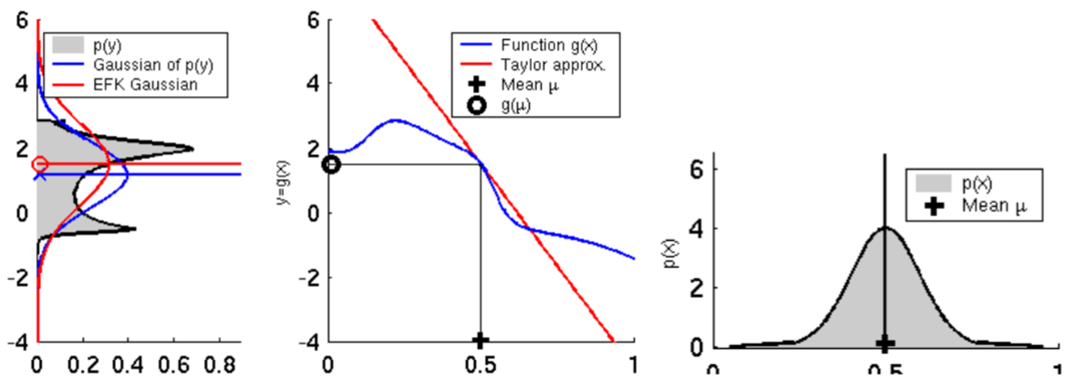
\includegraphics[width=0.9\linewidth, height=5cm]{scribe_EKFexamples} 
    \caption{EKF Examples}
    \label{fig:EKFexamples}
\end{figure}

\subsection{Unscented Kalman Filter}

\subsubsection{UKF Overview}
Another way to utilize Gaussian approximations, but without linearization, is the Unscented Kalman Filter. While the EKF propagates an entire Gaussian using a approximated motion and measurement models, the UKF approximates the current belief by selecting sigma-points, then uses the full non-linear model to propagate those points forward. This tends to mean that the UKF is a bit slower due to the need to process individual particles. However, it is more accurate and more robust in high variance situations. 

\subsubsection{UKF Set-up}
To implement the UKF, we first have to develop equations to compute relevant sigma points, find corresponding weights for those sigma points, and compute Gaussian parameters from a set of transformed points. Sigma points should be chosen symmetric relative to the eigenaxis of the uncertainty ellipse; the set of sigma points should contain at least the mean, as well as points some displacement along the axis. The equations for determining sigma points ($X^{[i]}$) and weights ($w_m^{[i]}, w_c^{[i]}$) are described below. Assume n-dimensional Gaussian $N(\mu,\Sigma)$

\par Sigma Points:
\begin{equation}
    X^{[0]} = \mu
\end{equation}
\begin{equation}
    X^{[i]} = \mu + (\sqrt{(n+\lambda)}\Sigma)_{i} \quad \txtrm{for} \quad i=1,...,n
\end{equation}
\begin{equation}
    X^{[i]} = \mu - (\sqrt{(n+\lambda)}\Sigma)_{i-n} \quad \txtrm{for} \quad i=n+1,...,2n
\end{equation}

Weights:
\begin{equation}
    \omega_{m}^{[0]}=\frac{\lambda}{n+\lambda}
\end{equation}
\begin{equation}
    \omega_{c}^{[0]}=\frac{\lambda}{n+\lambda}+(1-\alpha^{2}+\Beta) 
\end{equation}
\begin{equation}
    \omega_{m}^{[i]}=\omega_{c}^{[i]}=\frac{1}{2(n+\lambda)} \quad \txtrm{for} \quad i=1,...,2n
\end{equation}

Once the new points have been computed (see section \ref{sec:ukfalgo}), it is necessary to fit the new points to a Gaussian by recovering the mean and covariance:
\begin{equation}
    \mu' = \sum_{i=0}^{2n}\omega_{m}^{[i]}Y^{[i]}
\end{equation}
\begin{equation}
    \Sigma' = \sum_{i=0}^{2n}\omega_{c}^{[i]}(Y^{[i]}-\mu')(Y^{[i]}-\mu')^{T}
\end{equation}

\subsection{Algorithm}\label{sec:ukfalgo}
The UKF instantiates the Bayes filter with a prediction step and a correction step. The prediction step takes original sigma points $X_{t-1}$ and propagates them forward with the full dynamics model $Y^{[i]} = g(X^{[i]})$ to get resulting points $X_{t}^*$. These points are then fit to a Gaussian by recovering the mean and covariance.
$$X_{t-1}=(\mu_{t-1}, \mu_{t-1}+\gamma\sqrt{\Sigma_{t-1}}, \mu_{t-1}-\gamma\sqrt{\Sigma_{t-1}}$$
$$X_{t}^{*} = g(\mu_{t}, X_{t-1})$$
$$\overline{\mu_{t}} = \sum_{i=0}^{2n}\omega_{m}^{[i]}\overline{X_{t}^{*[i]}}$$
$$\overline{\Sigma_{t}} = \sum_{i=0}^{2n} \omega_{c}^{[i]}(\overline{X_{t}^{*[i]}}-\overline{\mu_{t}})(\overline{X_{t}^{*[i]}}-\overline{\mu_{t}})^{T}+R_{t}$$

The correction step accounts for measurements by approximating the predicted belief $X_{t}$ with sigma points. Then predict the measurements $Z_{t}$ for the sigma points using the nonlinear measurement model. Finally, reconstruct the Gaussian.
$$\overline{X_{t}} = \overline{\mu_{t}}, \overline{\mu_{t}}+\gamma\sqrt{\overline{\Sigma_{t}}}, \overline{\mu_{t}}-\gamma\sqrt{\overline{\Sigma_{t}}}$$
$$\overline{Z_{t}} = h(\overline{X_{t}})$$
$$\hat{z}_{t} = \sum_{i=0}^{2n}\omega_{m}^{[i]}\overline{Z_{t}^{[i]}}$$
$$S_{t} = \sum_{i=0}^{2n}\omega_{c}^{[i]}(\overline{Z_{t}^{[i]}} - \hat{z}_{t})(\overline{Z_{t}^{[i]}} - \hat{z}_{t})^{T}+Q_{t}$$
$$\overline{\Sigma_{t}^{x,z}} = \sum_{i=0}^{2n}\omega_{c}^{[i]}(\overline{X_{t}^{[i]}} - \mu_{t})(\overline{Z_{t}^{[i]}} - \hat{z}_{t})^{T}$$
$$K_{t} = \overline{\Sigma_{t}^{x,z}}S_{t}^{-1}$$
$$\mu_{t} = \overline{\mu_{t}}+K_{t}(z_{t} - \hat{z}_{t})$$
$$\Sigma_{t} = \overline{\Sigma_t}-K_{t}S_{t}K_{t}^{T}$$


\section{Non-Parametric Filters}\label{sec:nonparametric}
Non-Parametric Filters do not force assumptions upon what the belief should look like (e.g. Gaussian). This allows for more flexible belief spaces, such as multi-modal. However, it requires a certain amount of approximation to provide a computational simplification of the Bayes filter algorithm.

\subsection{Histogram Filters (Discrete Bayes Filter)}
Histogram filters use a discrete approximations of a continuous distributions, i.e. considering pmfs or histograms as opposed to pdfs.

Before the discrete Bayes' filter can be executed, several discretizations must be done. First, a (continuous) state space must be discretized into a finite number of bins/cells. Each state, $x_{k,t}$, is then assigned a probability, $p_{k,t}$, which represents the probability of being in a particular cell in the state space. For all $x_t \in x_{k,t}$,

\begin{equation}
    p(x_t) \equiv \frac{p_{k,t}}{|x_{k,t}|} 
\end{equation}

so these probabilities are assumed to be uniform. \\
Next, the motion and measurement models must also be discretized without taking into account the exact state we are in. To do this, we choose a \textit{mean state} $\hat{x}_{k,t}$ (which can be thought of as the central mass of the cell) as a representative state:

\begin{equation}
    \hat{x}_{k,t} = |x_{k,t}|^{-1}\int_{x_{k,t}} x_tdx_t
\end{equation}
And approximate the measurement and transition models using the mean state:
\begin{equation}
    p(z_t|x_{k,t})\approx p(z_t|\hat{x}_{k,t})
\end{equation}
\begin{equation}
    p(x_{k,t}|u_t, x_{k,t-1})\approx \eta |\hat{x}_{k,t}|p(\hat{x}_{k,t}|\hat{u}_t,\hat{x}_{k,t-1})
\end{equation}

The algorithm for the discrete Bayes' filter is essentially the same as the continuous Bayes' filter. The only difference is replacing the integrals with summations for each cell.

\subsection{Particle Filters}

The particle filter is another non-parametric implementation of Bayes' filter. Similar to the histogram filter, it approximates the posterior belief with a finite number of discrete parameters. In this case, a number of particles represents the posterior belief. This filter allows for both the use of nonlinear transformations and also the representation of non-Gaussian distributions, including multi-modal beliefs. 


For this filter, samples of particles (represented by vertical bars in Figure \ref{Particle Representation of Belief [2]}) represent the belief of state, where a higher density of particles corresponds to a higher belief that the state lies in a certain region. 


\begin{figure}[h]
    \begin{center}
    
    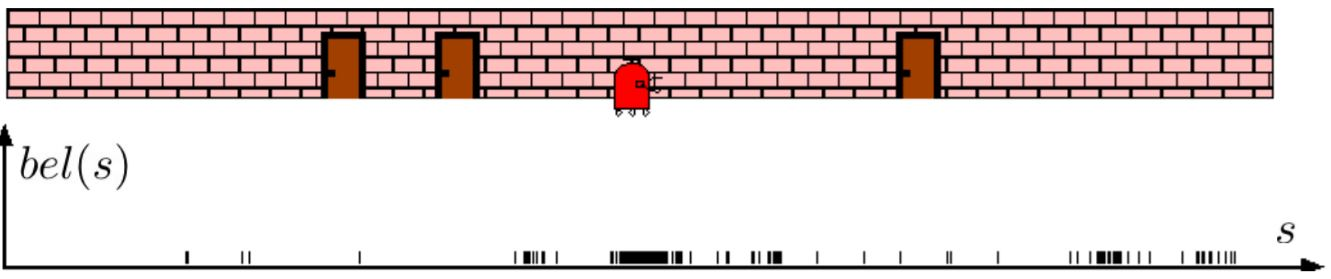
\includegraphics[width=0.9\linewidth, height=3cm]{particle_algorithm_pic} 
    \caption{Particle Representation of Belief [2]} 
    \label{Particle Representation of Belief [2]}
     \end{center}

\end{figure}

The belief is represented by a set of M particles: 

\begin{equation}
    \chi_t := x_t^{[1]},\  x_t^{[2]},\ .\ .\  . \ \ , \ x_t^{[M]} 
\end{equation} 

Each particle represents a hypothesis about what the true state could be. Ideally the particles are distributed according to the probability of the current state, given all measurements and control inputs up to that time: 

\begin{equation}
    x_t^{[m]} \sim  p(x_t \ |\ z_{1:t}, \ u_{1:t}) = bel(x_t) 
\end{equation} 

Maintaining such a series of particles for each time step allows us to fit a probability distribution across the particle samples to understand the belief of state. The particle filter algorithm recursively constructs a particle set at the current time from a particle set at the previous time step, with the goal that the new set matches the target posterior distribution.  In order to do so, the algorithm exploits principles from Bayesian filtering.   



\subsubsection{Algorithm}

The algorithm inputs are the particle representation of belief at the previous time step as well as the control and measurement of the current time step. The algorithm outputs another set of particles representing the posterior belief.  This algorithm can be broken down into two key components:

\begin{figure}[h]
    \begin{center}
    
    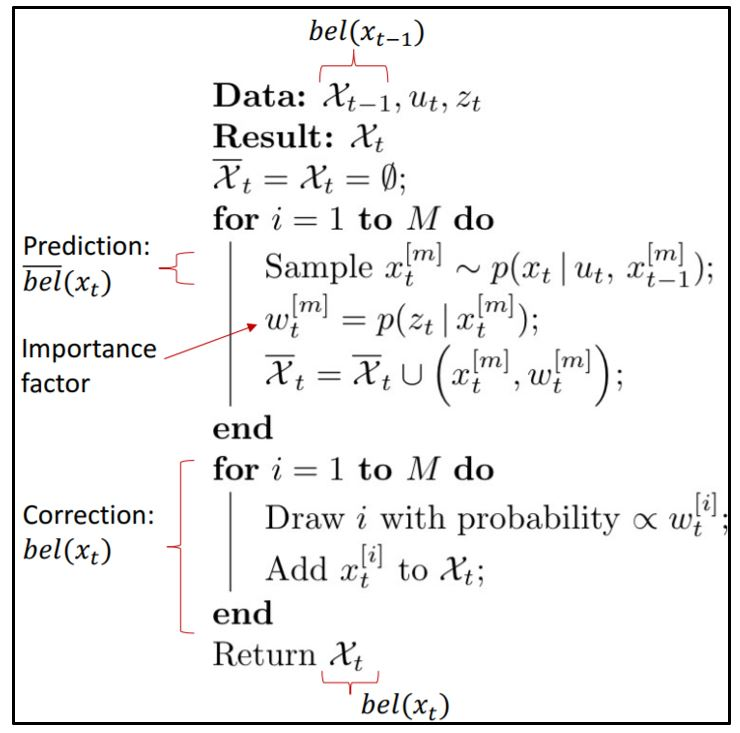
\includegraphics[width=0.5\linewidth, height=8cm]{particle_algorithm} 
    \caption{Particle Filter Algorithm [2]} 
    \label{fig: Particle Filter Algorithm (Lecture 11 Slides)}
     \end{center}

\end{figure}


\begin{enumerate}
    \item Prediction Step

    \begin{itemize}
        \item 
    
    The algorithm first uses the set of particles representing the prior belief along with the control input and state transition model to sample a new set of particles that represent the new belief for time t. 

        \item
    For each new particle that is sampled, a weight is computed (referred to as an importance factor), which represents the probability of that sampled particle given the observed measurement. 
        \item
    The set of sampled particles with corresponding importance factors represents the prediction belief and is passed on to the next part of the algorithm.
    
    \end{itemize}
\item Correction Step

 \begin{itemize}
        \item 
    The correction step draws particles from the prediction set, with probability matching the importance factor of each particle.  
        \item 
    This effectively ensures that particles in the prediction set that are deemed implausible by the current measurement are unlikely to make it into the final belief set, as these particles do not represent legitimate hypotheses for the state. This enforces that the final belief distribution complies with the observed measurement. 
    \end{itemize}

\end{enumerate}

After the prediction and correction resampling, if the number of total particles M approaches a very large number, the belief can be represented by the below equation. Typically, a value of roughly 1000 samples can adequately represent the posterior belief. 

\begin{equation}
    bel(x_t) = \eta  p(z_t \ |\ x_t^{[m]})\overline{bel}(x_t)  
\end{equation} 

The particle filter has certain computational benefits because of its process of using a subset of samples to represent a probability distribution. But there is a potential risk that the incomplete sampling of the belief distribution could lead to a robot losing an accurate representation of its true state, especially in the case where the robot receives accurate but unlikely measurement data [1]. 


%%%
%Figure 11.5 demonstrates how the resampling procedure reconciles the predicted belief set of particles with the measurement. 


%\begin{figure}[h]
%    \begin{center}
%    
%    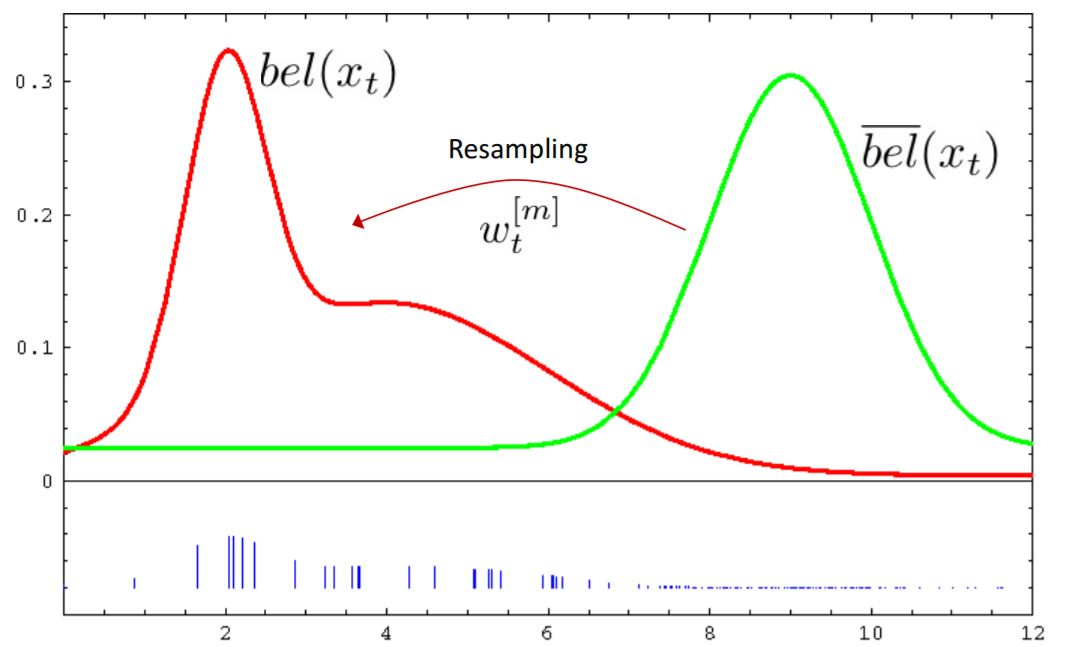
\includegraphics[width=0.7\linewidth, height=6cm]{particle_algorithm_pic2} 
%    \caption{Particle Filter Algorithm: Correction Step Diagram [2]} 
%    \label{fig: Particle Algorithm: Correction Step Diagram [2]}
%    \end{center}

%\end{figure}


\section{Localization Overview}
In order to select an appropriate filtering algorithm, we must consider the specifics of the problem.
For example, position tracking presents as a problem in which initial pose is known (i.e. there is little variance around the mean), so can be well-represented with one of the parametric filters discussed in Section \ref{sec:parametric}. Conversely, in a global localization problem, the initial state is unknown; the initial belief may be multimodal, and therefore these problems are better represented by one of the non-parametric filters in \ref{sec:nonparametric}. One example of global localization is called the "kidnapped robot" problem, where the robot is effectively teleported to another (unknown) location. This can be a helpful model for when our estimated state diverges from true state, and we need to reset the filter.
There are several other characteristics to consider when choosing a filtering algorithm:
\begin{itemize}
    \item Static environment (robot position is the only changing variable) vs.\\
    Dynamic environment (other moving objects exist in the environment)
    \item Passive localization (robot motion aims towards a goal unrelated to localization) vs.\\
    Active localization (actions explicitly made to reduce uncertainty in localization)
    \item Single-robot localization (individual robot only) vs.\\
    Multi-robot localization (team of robots engaged in cooperative localization)
\end{itemize}

Robot localization involves integrating data over time in order to determine the robot's position relative to a given map. In Lecture 10, we learned how to represent localization problems using the Markovian state assumption; we also learned about the Bayes' Filter Algorithm, which consists of a prediction step, followed by a taking a measurement and performing a correction update. The Bayes' Filter provides a general, but unsolvable, algorithm for localization. In Lecture 11, we introduced several different assumptions to make the filter tractable. The suitability of these assumptions relies on the specifications of the problem.


\begin{thebibliography}{9}

\bibitem{latexcompanion}
R. Siegwart, I. R. Nourbakhsh, D. Scaramuzza. \textit{Introduction to Autonomous Mobile Robots.} MIT Press, 2nd Edition, 2011.

\bibitem{latexcompanion}\label{bib:lecnotes}
Pavone, M. (2018). AA274: Principles of Robotic Autonomy, lecture 11 notes [PowerPoint Slides]. Retrieved from
https://canvas.stanford.edu/courses/75589/files/folder/Lectures

\bibitem{latexcompanion}
Chapter 4 Bayesian Decision Theory. www.byclb.com/TR/Tutorials/neural\_networks/ch4\_1.htm

\end{thebibliography}

\end{document}